\chapter{The Arrow, the Hours, and the Cliff}

In this School of Hard Knocks conversation, curated by LazyingArt LLC, the published video begins by showing us consequences before causes. We hear the sharp lines first: bad advice, money that turns into misery, giant years, celebrity scale. Only afterward do we arrive at the gate, the greeting, the ordinary human meeting that makes those lines answerable. From there the lecture unfolds in a disciplined sequence: one sharpened skill before many hats, time applied as a cumulative force, suffering as formation, confidence as the residue of tolerated failure, relationships as delayed structure, and finally the claim that the material summit has an abyss of its own.

\section{The Cold Open and the Real Meeting}

The lecture begins twice, and it is worth keeping that rhythm. First we get the compressed trailer version of the argument, almost as if the answers were known before the questions had been earned. Then the scene restarts in ordinary time: the gate, the walk-up, the greeting, the names, the easy talk, and the reintroduction of Will Smith not as an abstraction but as a person standing in front of us.

That duplication matters because it tells us how the lecture wants to move. It wants first to establish scale and pressure, and only then to disclose mechanism. The first blunt fact, when the conversation settles, is that Smith did not come from money. He says he came from ``the opposite.'' The point is not bookkeeping. The point is that the later claims about craft, judgment, freedom, and collapse are not offered as the inherited wisdom of comfort.

From there the host immediately does the right thing. He asks not merely who Smith is, but what route he took. Music leads to television, television to film, film to production and business. That visible plurality creates the chapter's first real puzzle. If the route contains many domains, why does the argument soon insist on one point of mastery?

\section{From Many Hyphens Back to One Point}

\paragraph{Anecdote.}
Smith's biography appears, at first glance, to be an argument for diversification. He has been a musician, an actor, a producer, and a businessman. The host sees that visible spread and asks whether a young operator should start by focusing or by scattering effort across ventures.

\paragraph{Claim.}
Smith's answer is sequential rather than ideological. He is not against later plurality. He is against premature plurality. The lecture's governing image is the arrow: one thing at the tip, done specifically and well, and only later the trailing body of other possibilities.

We can write the lecture's core construction as
\begin{align}
\text{mastery}(x_{\mathrm{tip}})
&\Longrightarrow
\text{expansion}(\mathcal D_{\mathrm{trail}}),\\
\text{one domain mastered}
&\Longrightarrow
\text{transferable comprehension of adjacent domains}.
\end{align}
Here \(x_{\mathrm{tip}}\) denotes the sharpened primary craft, and \(\mathcal D_{\mathrm{trail}}\) the later family of ventures that can follow once the tip has broken through.

\paragraph{Mechanism.}
The arrow does two pieces of work at once. First, it rejects the fantasy that many weak efforts add up to one strong one. Second, it explains how later diversification can be real rather than decorative. The later ventures are not independent ornaments. They are pulled behind a point that has already learned how to penetrate.

\begin{figure}[h]
\centering
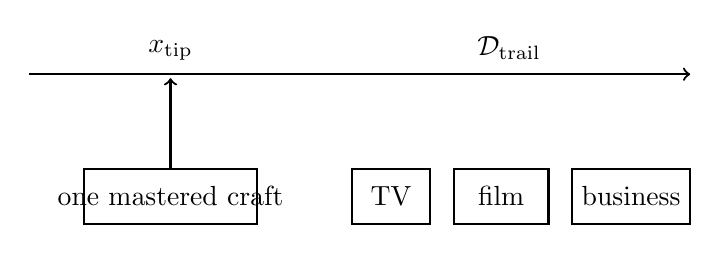
\begin{tikzpicture}[x=1cm,y=1cm,thick]
\draw[->] (0,0) -- (8.4,0);
\node[above] at (1.8,0.05) {$x_{\mathrm{tip}}$};
\node[above] at (6.1,0.05) {$\mathcal D_{\mathrm{trail}}$};

\draw (0.7,-1.2) rectangle (2.9,-1.9);
\node at (1.8,-1.55) {one mastered craft};
\draw[->] (1.8,-1.2) -- (1.8,-0.05);

\draw (4.1,-1.2) rectangle (5.1,-1.9);
\node at (4.6,-1.55) {TV};

\draw (5.4,-1.2) rectangle (6.6,-1.9);
\node at (6.0,-1.55) {film};

\draw (6.9,-1.2) rectangle (8.4,-1.9);
\node at (7.65,-1.55) {business};
\end{tikzpicture}
\caption{Transcript-derived arrow schematic. Smith's point is not that one must remain singular forever. It is that later plurality becomes powerful only after a real point has been sharpened.}
\end{figure}

The appeal to \emph{The Alchemist} strengthens the same thought. If the whole universe can be read through a grain of sand, then one deeply learned craft can become an epistemic base rather than a prison. Local mastery, in this lecture, is the condition for later breadth.

\subsection{Question \& Answer}

\paragraph{Question.}
Should we diversify early, or master one thing first?

\paragraph{Answer.}
The lecture answers by order rather than slogan. First the point, then the spread. A dull object with many attachments is not the same thing as a sharp object with direction. Smith's own career is not an excuse for early scattering; it is evidence that later expansion is strongest when it is pulled behind a genuine breakthrough.

\section{Time Applied Is Cumulative}

Once the argument has secured a direction, it asks the next question: what makes one competitor difficult to beat? Smith's answer is not mystical. He says the wind goes to the most hours committed. In other words, the decisive variable is not merely desire, nor even raw talent, but time applied steadily enough that it accumulates into a structural edge.

\paragraph{Claim.}
Time and attention are cumulative.

Let \(h\) denote committed hours per day and \(H(T)\) the cumulative hours invested over \(T\) days. The lecture's clean quantitative spine is then
\begin{equation}
H(T)=h\,T.
\end{equation}
For two operators \(A\) and \(B\), the cumulative gap after time \(T\) is
\begin{equation}
\Delta H(T)=\bigl(h_A-h_B\bigr)T.
\end{equation}

\paragraph{Mechanism.}
Smith's own example is simple: one person works \(10\) hours a day, another \(9\). Over a year,
\begin{align}
H_A(365)&=10\cdot 365,\\
H_B(365)&=9\cdot 365,
\end{align}
so that
\begin{align}
\Delta H(365)
&=H_A(365)-H_B(365)\\
&=(10-9)\cdot 365\\
&=365\ \text{hours}.
\end{align}
This is the worked example the chapter most needs. It converts motivational language into arithmetic without pretending that Smith is offering a universal theorem of outcomes. One extra hour per day sounds small locally. At yearly scale it is an additional \(365\) hours of contact with the craft.

A second way to see the same fact is through the ratio
\begin{equation}
\frac{H_A(365)}{H_B(365)}=\frac{10}{9}\approx 1.11.
\end{equation}
So the lecture's implicit claim is that a steady one-hour daily edge yields roughly an eleven-percent cumulative edge in applied time over the year.

We should keep the conclusion at the level Smith keeps it:
\begin{equation}
H_A(T)>H_B(T)
\Longrightarrow
\text{the catch-up problem for }B\text{ grows with }T.
\end{equation}
That is a practical rule, not a law of destiny. Talent still matters. Luck still matters. But the lecture is right to insist that many apparent differences in level are really differences in accumulated contact time.

The transition to the next section is important. Once time has been formalized as a force, the lecture asks what sort of being is applying that force. We move from the arithmetic of work to the structure of the worker.

\section{The Small Constellation, the Gift of Difficulty, and the Larger Energy}

The host shifts from career success to acting and asks what Smith has learned about people. The answer is not social psychology in the ordinary sense. It is a reduction of the ordinary self. What we call a person, Smith says, is often only a personality: a small constellation of ideas that we have chosen to live inside.

Let \(P\) denote that narrow personality-construct and \(S\) the larger self to which the lecture keeps pointing. Then the claim may be summarized as
\begin{equation}
P \subsetneq S.
\end{equation}
That is, the familiar identity is only a sliver of the possible person. Race, creed, color, city, and country are not nothing; but when we mistake them for the whole, they harden into prison bars. This is why the lecture does not treat identity as merely descriptive. It treats it as a limit on action.

The next question, through \emph{The Pursuit of Happyness}, is how such a self is shaped. Smith's answer, drawing on Chris Gardner, is severe and direct: suffering is a gift, difficulty is a teacher, adversity is where willpower and energy are formed. The point is not to glorify pain for its own sake. The point is that the lecture sees deep formation happening under pressure rather than in ease. In schematic form:
\begin{equation}
\text{difficulty}
\longrightarrow
\text{shaping of willpower and energy}
\longrightarrow
\text{greater usable force}.
\end{equation}
This is the right place for Smith's line about getting comfortable being uncomfortable. It is not a side remark. It is the practical form of the entire argument about suffering.

Faith enters next, and it enters in the same line of motion rather than as a separate sermon. Smith says he believes in a creative energy constantly at work in all things and that relation to this energy enlarges what he can do beyond the scale of the ego. The cleanest way to preserve that without over-formalizing it is
\begin{equation}
\text{creative capacity}_{\mathrm{ego}}
<
\text{creative capacity}_{\mathrm{aligned}}.
\end{equation}
His ``hundredfold'' language should be heard as rhetorical scale rather than literal multiplier. The chapter should remain faithful to that tone. The lecture is not offering theology in formal dress. It is saying that the agent who acts is larger than the ego's everyday enclosure, and that relation to that larger field alters the scale of creation.

At this point the lecture has not abandoned career reasoning. It has deepened it. The earlier account of hours and mastery now sits inside a larger account of the person who can withstand hours, survive difficulty, and avoid collapsing into a narrow self-story.

\section{Confidence in Its Seeds}

The next prompt, through \emph{Hitch}, asks about confidence. The host frames the problem in the most ordinary way: confidence and self-belief appear to separate those who succeed from those who freeze. Smith's answer is one of the best reversals in the interview. Confidence, he says, is not what it first appears to be.

\paragraph{Claim.}
Confidence is not initially a polished inner possession. It begins in the willingness to look stupid.

This matters because it relocates the source of visible confidence. The person who looks confident may simply be a person for whom public error has stopped being disqualifying. Smith says it plainly: it looks like confidence when you are not scared to fail, but it is not confidence in finished form. It is confidence in seed form.

\paragraph{Mechanism.}
The process the lecture describes can be written as
\begin{equation}
\text{attempt}
\longrightarrow
\text{public miss}
\longrightarrow
\text{survival}
\longrightarrow
\text{repetition}
\longrightarrow
\text{reduced fear}
\longrightarrow
\text{perceived confidence}.
\end{equation}
He gives one concrete performance ratio:
\begin{equation}
p_{\text{hit}}=\frac{3}{10}=0.3.
\end{equation}
This is not a statistical law. It is a way of making the lesson unforgettable. If three hits out of ten are enough to count as greatness, then the fear of not being perfect is not a rational guide to action.

\begin{figure}[h]
\centering
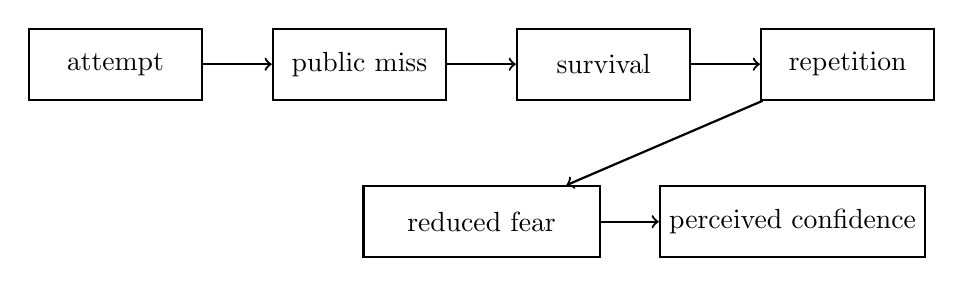
\begin{tikzpicture}[x=1cm,y=1cm,thick]
\node[draw, rectangle, minimum width=2.2cm, minimum height=0.9cm] (a) at (0,0) {attempt};
\node[draw, rectangle, minimum width=2.2cm, minimum height=0.9cm] (b) at (3.1,0) {public miss};
\node[draw, rectangle, minimum width=2.2cm, minimum height=0.9cm] (c) at (6.2,0) {survival};
\node[draw, rectangle, minimum width=2.2cm, minimum height=0.9cm] (d) at (9.3,0) {repetition};

\node[draw, rectangle, minimum width=3cm, minimum height=0.9cm] (e) at (4.65,-2) {reduced fear};
\node[draw, rectangle, minimum width=3.3cm, minimum height=0.9cm] (f) at (8.6,-2) {perceived confidence};

\draw[->] (a) -- (b);
\draw[->] (b) -- (c);
\draw[->] (c) -- (d);
\draw[->] (d) -- (e);
\draw[->] (e) -- (f);
\end{tikzpicture}
\caption{Transcript-derived confidence sequence. What later appears as confidence is built out of repeated contact with embarrassment, error, and recovery.}
\end{figure}

\paragraph{Anecdote.}
Smith locates this lesson in the practical world of performance, especially \emph{The Fresh Prince of Bel-Air}. One bad joke does not end the work. One wrong take does not end the work. The public sees surface ease; the lecture wants us to see its substrate.

\subsection{Question \& Answer}

\paragraph{Question.}
What is confidence actually made of?

\paragraph{Answer.}
It is made of tolerated embarrassment. More exactly, it is made of surviving enough visible failure that failure loses its veto power. The lecture therefore refuses the fantasy that confidence must come first. Very often it is the name we give, afterward, to a person who has become less frightened of looking foolish.

\section{Advice, Intuition, and the Network of Return}

Once fear has lost some of its veto power, the next problem is judgment. Whose voice do we allow into the work? Smith returns here to one of the lines that appeared in the cold open: taking advice from somebody who has not done what we want to do is almost insanity.

We may write the lecture's advice filter as
\begin{equation}
\mathcal A
=
\{x:\ x \text{ has actually done what we seek to do}\}.
\end{equation}
The admissible set is small. That is the point. The lecture is not anti-advice in general; it is anti-undisciplined exposure to opinions that have not been tested in the field one actually cares about.

The Quincy Jones story gives the claim its mature form. Smith asks for advice. Quincy refuses to counterfeit omniscience about a path he would not have chosen himself. That refusal becomes a deeper form of help than a generic answer would have been. The lecture then moves one step further: eventually one asks for advice less, watches more, and lets behavior speak.

That progression ends in the bird-and-branch analogy:
\begin{equation}
\text{trust}(\text{wings})>\text{trust}(\text{branch}).
\end{equation}
This is only a schematic rendering of the image, but it captures the point. A branch may be strong or weak. A life built only on branches remains fragile. The bird survives because it carries a means of re-stabilization within itself.

The published interview then breaks for a long promotional interruption. When it returns, it returns not to money but to mentors and relationships. Smith remembers his grandmother's warning: everywhere you go, one day you may have to go back. This becomes a long-horizon theory of social value. The lecture's own timeline is explicit:
\begin{equation}
16
\Longrightarrow
24
\Longrightarrow
34.
\end{equation}
The sixteen-year-old we meet now may be running a company at twenty-four and tied into our family or institution by thirty-four. In other words, relationships are not static. They evolve in role, relevance, and consequence.

The lecture's practical summary is severe and memorable: people will take you places money cannot. That is not a sentimental slogan. It is a statement about the structure of future opportunity.

Only after that social doctrine does the host bring the conversation back to financial freedom. Smith's answer loops us back to the arrow. Sometimes, he says, what we like is different from what we are best at. In our notation:
\begin{equation}
\text{preference}\neq\text{comparative advantage}.
\end{equation}
He loved music. He says he was better as an actor. The turning point came when he chose the stronger craft and allowed money to arrive behind mastery rather than in front of it:
\begin{equation}
\text{mastery in the strongest craft}
\Longrightarrow
\text{finance follows behind mastery}.
\end{equation}
This is one of the lecture's most valuable returns. The earlier principle about the arrow is not abandoned after the social section. It comes back as the actual turning point.

\section{Money, Misery, and the Corresponding Abyss}

Smith does not answer the question about the largest annual dollar figure directly. He avoids the number, but he does identify a peak creative and financial interval: \emph{Hancock} and \emph{I Am Legend} arriving within roughly six months of each other. The detail matters because it keeps the scale concrete without turning the chapter into a vanity ledger.

From there the lecture returns to one of its opening provocations: money does not buy happiness. More sharply, there is a level beyond which it begins to buy misery. Smith gives a rough American marker,
\begin{equation}
m_\ast \approx \$1{,}000{,}000/\text{year},
\end{equation}
and the notes should preserve it exactly in that spirit: as Smith's own heuristic rather than a general economic law. The sign change he has in mind is social and existential before it is statistical. Up to a point, money relieves real constraints. Past a point, it alters the social field around the person.

In the lecture's own spirit we can write
\begin{align}
m \uparrow
&\Longrightarrow
\text{constraint relief, up to a point},\\
m \gtrsim m_\ast
&\Longrightarrow
\text{new suspicion, distortion, and attack.}
\end{align}
This is why the lecture says that at certain financial levels it becomes harder to make new friendships. People begin to think about the money. The person becomes socially over-read. Wealth changes sign.

The host then introduces the deepest late image of the interview: clifftop versus rock bottom. We normally assume that change comes at the bottom. Smith says there is a corresponding upper abyss. One can have enough money, enough sex, enough fame, enough acquisition, and still reach an edge where nothing material any longer promises satisfaction. The symmetry may be written, schematically, as
\begin{equation}
\mathcal A_{\mathrm{rock\ bottom}}
\sim
\mathcal A_{\mathrm{clifftop}}.
\end{equation}
This is not an equivalence in any strict analytic sense. It is a faithful compression of the lecture's claim that deprivation and saturation can expose the same deeper lack.

\begin{figure}[h]
\centering
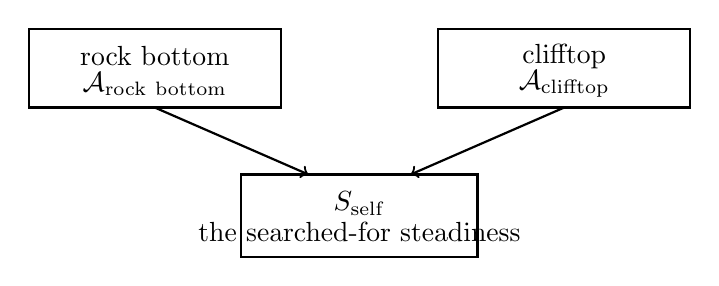
\begin{tikzpicture}[x=1cm,y=1cm,thick]
\draw (0,0) rectangle (3.2,1);
\node at (1.6,0.65) {rock bottom};
\node at (1.6,0.3) {$\mathcal A_{\mathrm{rock\ bottom}}$};

\draw (5.2,0) rectangle (8.4,1);
\node at (6.8,0.65) {clifftop};
\node at (6.8,0.3) {$\mathcal A_{\mathrm{clifftop}}$};

\draw (2.7,-1.9) rectangle (5.7,-0.85);
\node at (4.2,-1.22) {$S_{\mathrm{self}}$};
\node at (4.2,-1.58) {the searched-for steadiness};

\draw[->] (1.6,0) -- (3.55,-0.85);
\draw[->] (6.8,0) -- (4.85,-0.85);
\end{tikzpicture}
\caption{Transcript-derived symmetry of the two abysses. Poverty and saturation are not the same condition, but both can reveal that material arrangement is not identical with inner stability.}
\end{figure}

Smith's resolution is blunt. What one is actually looking for, beneath both extremes, is oneself. More precisely, one is looking for a steadiness that does not depend on branch strength. Money cannot cure every disease, repair every broken relationship, or prevent death. The branch can be strong or weak. The deeper question is whether the wings are real.

\subsection{Question \& Answer}

\paragraph{Question.}
Why can success become its own kind of cliff?

\paragraph{Answer.}
Because the material program can be completed without delivering the thing it promised. Rock bottom says: we do not have enough. Clifftop says: enough was not the thing we were actually after. The lecture's late movement insists that both discoveries are painful and that both drive us toward the same harder search for self-stability.

The closing message to younger listeners now lands with full force. Consciousness, Smith says, is an extraordinary tool of creation. One does not have to remain in the present job, city, or relationship merely because it is present. But the lecture refuses cheap liberation rhetoric. The price of exercising that freedom is willingness to suffer. Possibility is wide; enactment is costly.

\section{Summary}

This chapter moves from public success to the structure beneath it. We begin with the cold-open claims and then let the actual meeting earn them. We are shown why many hats should not be read as permission for early scattering, why the tip of the arrow matters more than the width of the trail, why hours accumulate into force, why personality can become prison, why suffering and faith enlarge the usable self, why confidence is built out of visible misses, why advice must be filtered by proof and eventually by intuition, why relationships are long-horizon infrastructure, and why money can both relieve constraint and deepen distortion.

The argument ends where the lecture wants it to end: not with the size of the career, but with the stability of the self. The arrow explains how one breaks through. The arithmetic of hours explains how one becomes hard to beat. The cliff explains why neither of those is yet the same as peace.